\chapter{Arsitektur MVVM (Model-View-ViewModel)}
\authors{Alfa Yohannis}

\section{Latar Belakang}
Pada mulanya, dalam pengembangan perangkat lunak, kode yang bertanggung jawab terhadap data, logika bisnis, dan tampilan (Graphical User Interface) bercampur jadi satu, tidak ada pemisahan abstraksi.
Pola Model-View-Controller kemudian muncul memisahkan kode program ke dalam 3 abstraksi utama berdasarkan perhatian mereka: \textit{model} untuk data, \textit{view} untuk tampilan, dan \textit{controller} untuk logika bisnis. 
Hanya saja, MVC tidak memiliki abstraksi yang secara eksplisit mengelola \textit{states} dari tampilan (\textit{views}).
Pola MVP (Model-View-Presenter) kemudian diajukan di mana komponen \textit{Presenter}-nya bertanggung jawab mengelola logika presentasi dari \textit{views}. Walaupun demikian,kode program yang mengelola sinkronisasi antara views dan state dari logika presentasi mereka masih harus dibuat secara manual.

Keunikan dari Model-View-ViewModel adalah pola tersebut memiliki komponen \textit{binder} yang mengotomasi komunikasi/sinkronisasi antara view dengan properties yang ada pada \textit{view model}. Nilai-nilai pada \textit{view} ditautkan dengan properties pada view model sehingga perubahan nilai pada salah komponen di view (misalnya perubahan pada \textit{textbox}) akan memperbarui juga nilai pada \textit{property}-nya di \textit{view model} yang ditautkan pada komponen tersebut. Adanya binder mengurangi jumlah kode yang harus ditulis oleh developer secara manual untuk melakukan sinkronisasi antara \textit{view} dan \textit{view model}.

\begin{figure}[h]
    \centering
    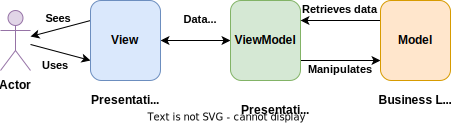
\includegraphics[width=\textwidth]{mvvm}
    \caption{Arsitektur Model-View-ViewModel (MVVM).}
    \label{fig:mvvm}
\end{figure}


\section{Arsitektur Model-View-ViewModel}
\begin{itemize}
\item Separation of the view layer by moving all GUI code to the view model via data binding.
\item UI developers don't write the the GUI, instead a markup language is used.
\item The separation of roles allows UI designers to focus on the UX design rather than programming of the business logic. 
\item A proper separation of the view from the model is more productive, as the user interface typically changes frequently and late in the development cycle based on end-user feedback.
\item Data bindings and properties are used to synchronise the relevant values in the view and the view model, that represents the state of the view, so that they are always the same.
\item It eliminates or minimises application logic that directly manipulates the view. 

\end{itemize}



\section{Kelebihan dan Kekurangan}
Berikut adalah kelebihan dan kekurangan arsitektur MVVM:


\subsection{Kelebihan}
Keuntungan dari menerapkan arsitektur MVVM adalah:
\begin{itemize}
\item Separation of the view layer by moving all GUI code to the view model via data binding.
\item UI developers don't write the the GUI, instead a markup language is used.
\item The separation of roles allows UI designers to focus on the UX design rather than programming of the business logic. 
\item A proper separation of the view from the model is more productive, as the user interface typically changes frequently and late in the development cycle based on end-user feedback.
\item Data bindings and properties are used to synchronise the relevant values in the view and the view model, that represents the state of the view, so that they are always the same.
\item It eliminates or minimises application logic that directly manipulates the view. 

\end{itemize}

\subsection{Kekurangan}
Konsekuensi dari penerapan arsitektur MVVM adalah sebagai berikut:
\begin{itemize}
\item It can be overkill for small projects. 
\item Generalizing the viewmodel upfront can be difficult for large applications.
\item Large-scale data binding can lead to lower performance.
\item It's best for UI development but might not the best for other types of developments and  applications.
\end{itemize}

\section{Contoh Kasus}

\subsection{Deskripsi}
Jelaskan contoh kasus yang dipaparkan berkaitan dengan arsitektur yang dimaksud pada bab ini.
Contoh kasus harus memperjelas arsitektur yang dimaksud.

\subsection{Penjelasan Implementasi}
Jelaskan bagian-bagian kode program, basisdata, atau konfigurasi yang signifikan terhadap arsitektur yang dimaksud.

\begin{lstlisting}[firstnumber=1,style=java,caption={Model dari \textsf{Rate}.},label=lst:rate_model]
import javax.persistence.Entity;
import javax.persistence.Id;
import javax.persistence.IdClass;

@Entity
@IdClass(RateId.class)
public class Rate {
  @Id
  private String fromCurrency;
  @Id
  private String toCurrency;
  private Double rate;
  ...
  Rate(String fromCurrency, String toCurrency, Double rate) {
    ...
  }
  ...
}
\end{lstlisting}

\begin{lstlisting}[firstnumber=1,style=java,caption={ \textsf{RateRepository}.},label=lst:rate_repository]
import java.util.Collection;
import org.springframework.data.jpa.repository.Query;
import org.springframework.data.repository.CrudRepository;

public interface RateRepository extends CrudRepository<Rate, Integer> {  
  @Query("SELECT r FROM Rate r WHERE r.fromCurrency = ?1 and r.toCurrency = ?2")
  Collection<Rate> findFirstByFromCurrencyAndToCurrency(String fromCurrency, String toCurrency);
  
  @Query("SELECT DISTINCT(r.fromCurrency) FROM Rate r")
  Collection<String> findAllFromCurrency();
  
  @Query("SELECT DISTINCT(r.toCurrency) FROM Rate r")
  Collection<String> findAllToCurrency(); 
}
\end{lstlisting}


\section{Kesimpulan}
Rangkum dan ulangi (beri penekanan pada) hal-hal kunci dari arsitektur yang dimaksud.